150. \begin{figure}[ht!]
\center{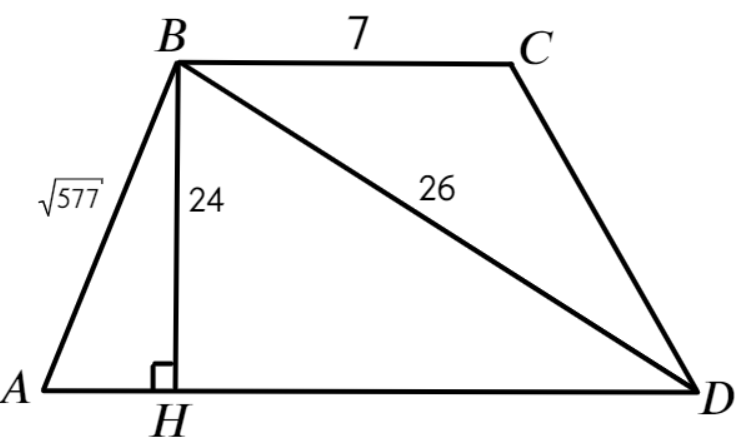
\includegraphics[scale=0.35]{g8-150.png}}
\end{figure}\\
По теореме Пифагора найдём $AH=\sqrt{(\sqrt{577})^2-24^1}=1$см, $HD=\sqrt{26^2-24^2}=10$см. Тогда $S_{ABCD}=BH\cdot \cfrac{BC+AD}{2}=24\cdot\cfrac{7+1+10}{2}=216\text{ см}^2.$\\
